\section{Differentials \& Taylor-Formula}

The differential of a function at a specific input value $x_0$ is
$df(x_0) = f'(x_0)\ dx$ and has the rules
\begin{enumerate}
    \item \emph{Linearity:} $d(\alpha u \pm \beta v) = \alpha d(u)\pm \beta d(v)\quad(\alpha, \beta \in \mathbb{R})$
    \item \emph{Product:} $d(uv) = ud(v)+vd(u)$
    \item \emph{Quotient:} $d(u\div v) = (vd(u) - ud(v))\div v^2$
    \item \emph{Chain rule:} $d(v \circ u) = (v'\circ u)d(u)$
    \item \emph{Inversion:} $d(u^{-1}(y))=\frac{1}{u'(x)}dy\quad(x=u^{-1}(y))$
\end{enumerate}

\subsection{Univariate Taylor Formula}

If $y=f(x)$ is defined on the interval $I=[x0,x_0+h=x]$
\begin{align*}
    f(x_{0}+h) & =
    f(x_{0})+\frac{1}{1!} f^{(1)}(x_{0})h + \frac{1}{2!}f^{(2)}(x_{0})h^{2} + \cdots \\
    & + \frac{1}{n!}f^{(n)}(x_{0})h^{n}+R_{n}(x_{0},h)
\end{align*}

With the remainder error term $R_n(x_0, h)$:
\begin{itemize}
    \item{
        \emph{Lagrange form:}
        \begin{align*}
            \frac{h^{n+1}}{(n+1)!} f^{(n+1)}({\underbrace{x_{0}+\vartheta\cdot h}_{\xi}})
            \ \ {\color{gray} (\xi\in(x_{0},x_{0}+h),\ \vartheta\in(0,1)\,)}
        \end{align*}
    }
    \item{
        \emph{Cauchy form:}
        \begin{align*}
            \frac{h^{n}(1-\vartheta)^{n}}{n!}f^{(n+1)}(\underbrace{x_0+\vartheta\cdot h}_\xi)
            \ {\color{gray} (\xi\in(x_0,x_0+h), \vartheta\in(0,1))}
        \end{align*}
    }
\end{itemize}

\subsection{Multivariate Taylor Formula}

\begin{align*}
    f(\vec{x}_0 + \vec{h}) = &
    \overbrace{f(\vec{x}_0) + \frac{1}{1!}\vec\nabla f(\vec{x}_0)\cdot \vec{h}}^{\text{Linear approximation}} \\
    & + \underbrace{\sum_{|\alpha|=2}^N\frac{1}{\alpha!}\frac{\partial^{|\alpha|}f(\vec{x}_0)}{\partial x^\alpha}\vec{h}^\alpha}_{\text{Higher order deriv.}}
    + \underbrace{\sum_{|\alpha|=N+1}R_\alpha(\vec{x}_0,\vec{h})\vec{h}^\alpha}_{\text{Reminder term}}
\end{align*}

where the reminder terms are absolutely bounded by
$\displaystyle\max_{\vec{x}\in S}\left| \frac{1}{\alpha!}\frac{\partial^\alpha f(\vec{x})}{\partial x^\alpha} \right|$
with $|\alpha|=N+1$ and
$S={\vec{x}}_{0}+\left(\left[-h_{1},h_{1}\right]\times\left[-h_{2},h_{2}\right]\times\cdots\times\left[-h_{n},h_{n}\right]\right)$
is an $n$-dimensional ``rectangle'' at center $\vec{x}_0$.


\section{Jacobian}

For each vector-valued function
$\vec{f} : \mathbb{R}^n \mapsto \mathbb{R}^m : \vec{y} = \vec{f}(\vec{x}) = \left(f_1(\vec{x}),f_2(\vec{x}),\ldots,f_m(\vec{x})\right)$
we can find a Jacobian matrix with the rows being the gradients $\vec{\nabla}f_j$:
\begin{snugshade*}
    \begin{align*}
        J_f(\vec{x}) = \begin{bmatrix}
                           \frac{\partial f_1(\vec{x})}{\partial x_1} &
                           \frac{\partial f_1(\vec{x})}{\partial x_2} &
                           \ldots &
                           \frac{\partial f_1(\vec{x})}{\partial x_n} \\
                           \frac{\partial f_2(\vec{x})}{\partial x_1} &
                           \frac{\partial f_2(\vec{x})}{\partial x_2} &
                           \ldots &
                           \frac{\partial f_2(\vec{x})}{\partial x_n} \\
                           \vdots & \vdots & \ddots & \vdots \\
                           \frac{\partial f_m(\vec{x})}{\partial x_1} &
                           \frac{\partial f_m(\vec{x})}{\partial x_2} &
                           \ldots &
                           \frac{\partial f_m(\vec{x})}{\partial x_n}
        \end{bmatrix}_{\color{gray}m\times n}
    \end{align*}
\end{snugshade*}


in the case of the Jacobian matrix being a square matrix ($m=n$), it has a determinant $\det(J_f(\vec{x}))$.
The determinant of a linear transformation A (square matrix) allows the computation of ``transformed volumes'':
$\mathrm{vol}(A(C))=|\det(A)|\mathrm{vol}(C)$, meaning for $y_j = f_j(x_1,\ldots,x_n)\quad(j=1,...,m=n)$:
\begin{align*}
    \underbrace{dy_1dy_2\cdots dy_n}_\text{transformed volume element} = \det(J_f(\vec{x}))
    \underbrace{dx_1dx_2\cdots dx_n}_\text{volume element}
\end{align*}

(requiring that $J_f$ is regular/invertible, i.e. $\det_{J_f}\neq0$)

\makebox[\columnwidth]{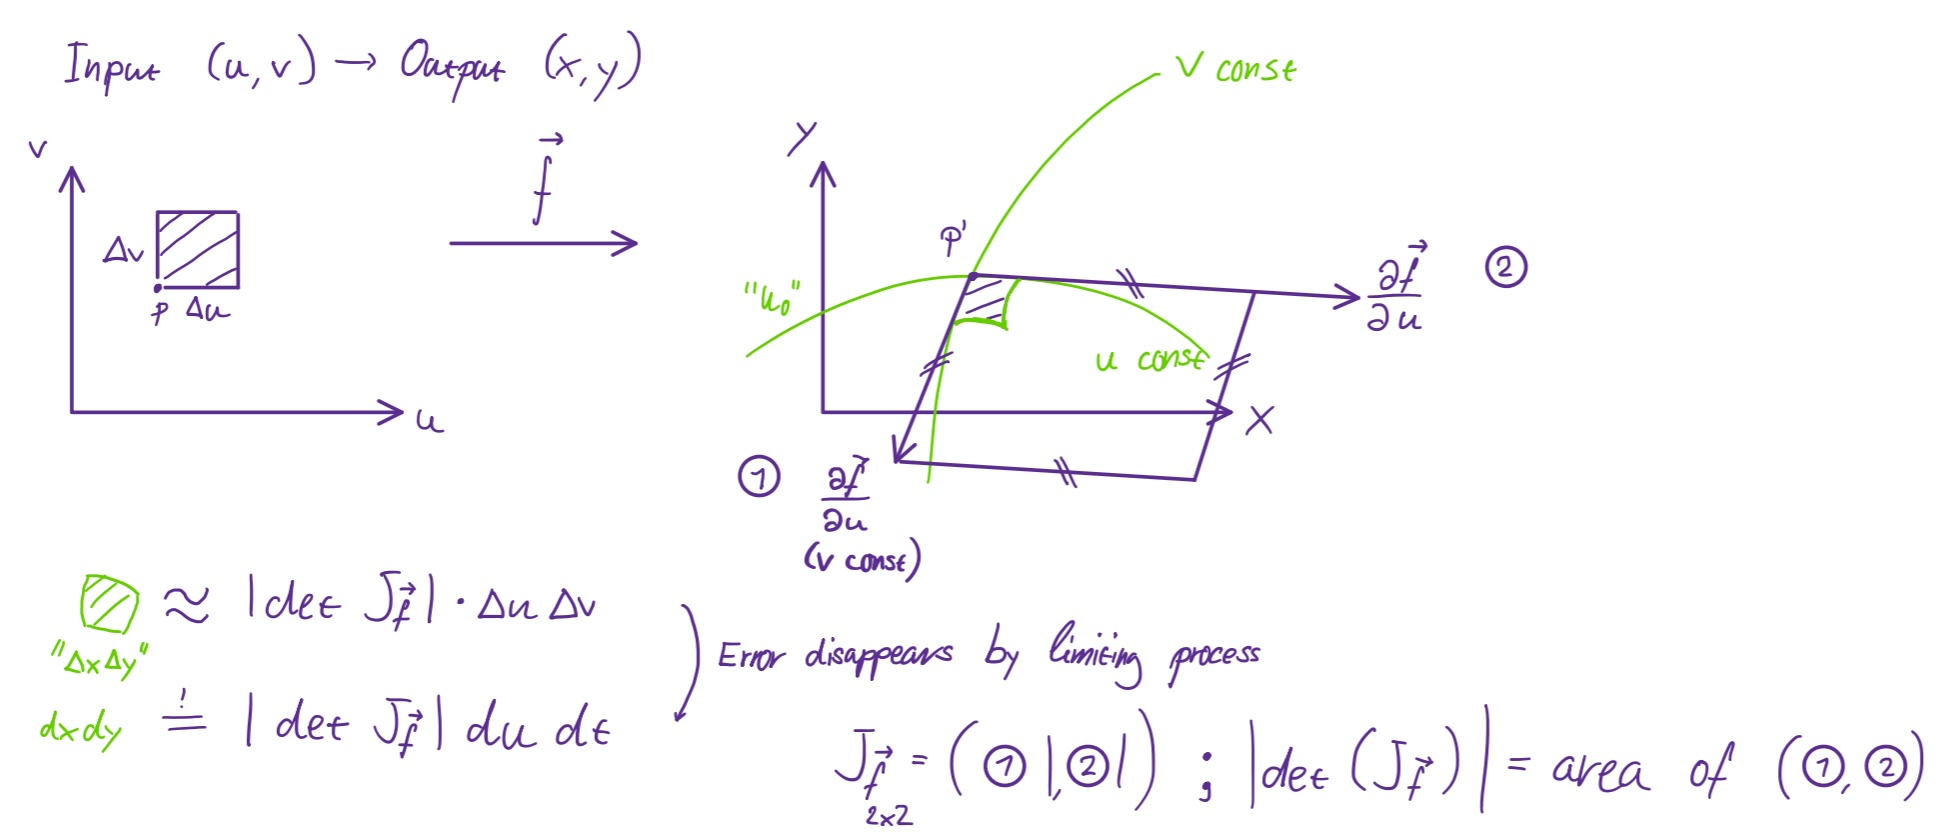
\includegraphics[width=\columnwidth]{images/jacobian}}

We therefore can do $\iint f(g(u,v), h(u,v))\det_J\ dudv$ when calculating a volume in $x,y$ using functions
$x=g(u,v)$ and $y=h(u,v)$ and the respective determinant of the transformation jacobian.

\textbf{For Example:} We want to compute the following integral on $\mathbb{R}^2$:
\begin{align*}
	\iint_{\mathbb{R}^2}e^{-\frac{x^2+y^2}{2}}\ dxdy
\end{align*}

by transformation to polar coordinates $(r,\varphi)$.
Hence, we have the transformation T: $(r,\varphi) \mapsto_T (x,y)$ with
\begin{align*}
	T(r,\varphi) = \begin{bmatrix}
		r\cos(\varphi) \\
		r\sin(\varphi)
	\end{bmatrix}
	=
	\begin{bmatrix}
		x(r, \varphi) \\
		y(r, \varphi)
	\end{bmatrix}
\end{align*}

and the Jacobian matrix:
\begin{align*}
	J_T =
	\begin{bmatrix}
		\frac{\partial x}{\partial r} & \frac{\partial x}{\partial \varphi} \\
		\frac{\partial x}{\partial r} & \frac{\partial x}{\partial \varphi}
	\end{bmatrix}
	=
	\begin{bmatrix}
		\cos(\varphi) & -r\sin(\varphi) \\
		\sin(\varphi) & r\cos(\varphi)
	\end{bmatrix}
\end{align*}

with the determinant $\det(J_T) = r\cos^2(\varphi) + r\sin^2(\varphi) = r$.
The transformed integral therefore looks like this:
\begin{align*}
	& \iint_{\mathbb{R}^2}e^{-\frac{x^2+y^2}{2}}\ dxdy \Rightarrow
	\int_0^{2\pi}\int_0^\infty e^{-\frac{\color{blue}r^2(\sin^2(\varphi)+\cos^2(\varphi))}{2}}{\color{purple}\det J_T}\ drd\varphi \\
	& = \int_0^{2\pi}\left(\int_0^\infty e^{-\frac{\color{blue}r^2}{2}}{\color{purple}r}\ dr\right)d\varphi 
	= \int_0^{2\pi} \left[ -e^{-\frac{r^2}{2}} \right]^\infty_0\ d\varphi \\
	& = \int_0^{2\pi} 1\ d\varphi = [\varphi]^{2\pi}_0 = 2\pi
\end{align*}
